% !TeX root = ../tesis.tex


\chapter{Ajuste con SSKKK}

\label{section:apendix2}

En la Sección \ref{section:optical_properties} se obtuvo la parte real de la función dieléctrica de los eritrocitos y el plasma a tra vés de la aplicaicón de las relaciones SSKK. En esta sección se mostrarán la aplicación de estas relaciones. En la Fig. se muestra la comparación entre la parte real de la función dieléctrica reconstruida mediante SSKK, indicada mediante la línea azul continua, y los datos experimentales para las concentraciones de hemoglobina de 15.3 g/dl y 28.7 g/dL indicados mediante los puntos rojos, observándose una desviación promedio de 0.003 y de , respectivamente. La línea continua que se observa es únicamente una guía al ojo. 
%
\begin{figure}[h]
	\centering
	
	\includegraphics[width=0.45\textwidth]{../../Figuras/ajusteLorentzLegend.pdf}\\
	\sidesubfloat[First image]{\hspace{-0.8cm}{
			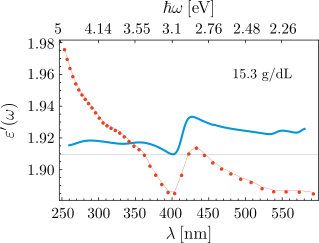
\includegraphics[width=0.47\textwidth]{../../Figuras/sskk15_0.pdf}\label{subfig:ajusteLorentz15}}}\hspace{0.1cm}
	\sidesubfloat[Second image]{\hspace{-0.6cm}{		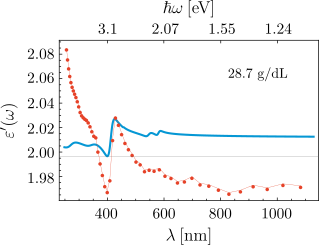
\includegraphics[width=0.47\textwidth]{../../Figuras/sskk28_0.pdf}\label{subfig:ajusteLorentz28}}}	
	\caption{Parte imaginaria de la función dieléctrica como función de la longitud de onda $\lambda$ (eje inferior) y la energía $\hbar\omega$ (eje superior). Se grafican datos experimentales representados por puntos rojos y el ajuste con lorenzianas con una línea azul continua para \textbf{a)} eritrocitos con una concentración de 15.3 g/dL, cuyos experimentales se obtuvieron de \cite{friebelDeterminationComplexRefractive2005a} y \textbf{b)} eritrocitos con una concentración de 28.7 g/dL, cuyos experimentales se obtuvieron de \cite{friebelModelFunctionCalculate2006}. En todas las figuras las líneas grises verticales indican las frecuencias de resonancia asociadas a los osciladores de Lorentz empleados en el ajuste.}
	\label{fig:epsLorentz1}
\end{figure}
%

De manera análoga, la Fig. \ref{subfig:epsSSKK_Plasma} muestra la parte real de la función dieléctrica obtenida mediante el análisis de SSKK como una línea azul continua, donde se observa una desviación promedio de 0.015 respecto a los datos experimentales (puntos rojos)

\begin{figure}[]
	\centering
	
	\sidesubfloat[Second image]{\hspace{-0.6cm}{		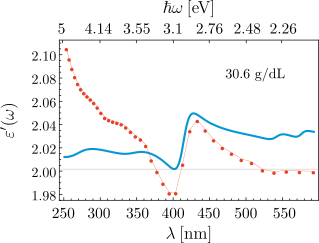
\includegraphics[width=0.5\textwidth]{../../Figuras/sskk30_0.pdf}\label{subfig:ajusteLorentz30}}}\hspace{0.1cm}
	\sidesubfloat[Second image]{\hspace{-0.8cm}{		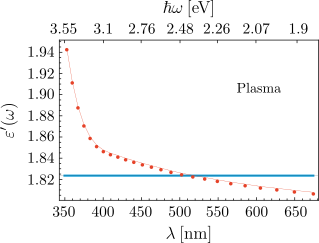
\includegraphics[width=0.47\textwidth]{../../Figuras/sskkPlasma_0.pdf}\label{subfig:ajusteLorentzPlasma}}}
	
	\caption{Parte imaginaria de la función dieléctrica como función de la longitud de onda $\lambda$ (eje inferior) y la energía $\hbar\omega$ (eje superior). Se grafican datos experimentales representados por puntos rojos y el ajuste con lorenzianas con una línea azul continua para \textbf{a)} eritrocitos con una concentración de 15.3 g/dL, cuyos experimentales se obtuvieron de \cite{friebelDeterminationComplexRefractive2005a}; \textbf{b)} eritrocitos con una concentración de 28.7 g/dL, cuyos experimentales se obtuvieron de \cite{friebelModelFunctionCalculate2006}; \textbf{c)} eritrocitos con una concentración de 30.6 g/dL, cuyos experimentales se obtuvieron de \cite{friebelDeterminationComplexRefractive2005a} y \textbf{d)} plasma, cuyos datos experimentales  se extrajeron de \cite{meinkeOpticalPropertiesPlatelets2007a}. En todas las figuras las líneas grises verticales indican las frecuencias de resonancia asociadas a los osciladores de Lorentz empleados en el ajuste.}
	\label{fig:epsLorentz2}
\end{figure}
%